\section{Representation and interpretation}

\subsection{Quality of the reconstruction}

\begin{frame}
  \frametitle{Contribution of each axis and quality of the representation}
  
  $\Delta_k$ is carrying inertia/variance defined by its orthogonal, thus 
  \begin{equation*}
      I_T = I_{\Delta_1^\bot} + \dots + I_{\Delta_p^\bot} = \lambda_1 + \dots + \lambda_p
  \end{equation*}

  \begin{block}{Relative contribution of axis $k$}<2->
    \vspace{-.5cm}
  \[ 
    \mathrm{contrib}(\Delta_k) = \frac{\lambda_k}{\sum_{k=1}^p\lambda_j} = \frac{\lambda_k}{\trace{\hat\bSigma}} \times 100 
  \]
    $^\rightsquigarrow$ \alert{Percentage of explained inertia/variance explained}
  \end{block}

  \begin{block}{Global quality of the representation on the first $k$ axes}<3->
    \vspace{-.5cm}
  \[ 
    \mathrm{contrib}(\Delta_1,\dots,\Delta_k) = \frac{\lambda_1 + \dots + \lambda_k}{\trace{\hat\bSigma}}  \times 100 
  \]
    A few axes may explain a large proportion of the total variance.\\
    $\rightsquigarrow$ \alert{This paves the way for dimension reduction} 
  \end{block}
  
\end{frame}

\begin{frame}[fragile]
  \frametitle{Scree plot: 'crabs'}

\begin{knitrout}
\definecolor{shadecolor}{rgb}{0.969, 0.969, 0.969}\color{fgcolor}\begin{kframe}
\begin{alltt}
\hlstd{crabs_pca} \hlkwb{<-} \hlkwd{select}\hlstd{(crabs,} \hlopt{-}\hlstd{species,} \hlopt{-}\hlstd{sex)} \hlopt \hlstd{FactoMineR}\hlopt{::}\hlkwd{PCA}\hlstd{(}\hlkwc{graph} \hlstd{=} \hlnum{FALSE}\hlstd{)}
\end{alltt}


{\ttfamily\noindent\bfseries\color{errorcolor}{\#\# Error in select(crabs, -species, -sex) \%>\% FactoMineR::PCA(graph = FALSE): could not find function "{}\%>\%"{}}}\begin{alltt}
\hlkwd{fviz_eig}\hlstd{(crabs_pca)}
\end{alltt}


{\ttfamily\noindent\bfseries\color{errorcolor}{\#\# Error in fviz\_eig(crabs\_pca): could not find function "{}fviz\_eig"{}}}\end{kframe}
\end{knitrout}

\end{frame}

\subsection{Individuals point of view}

\begin{frame}
  \frametitle{Individuals: representation in the new basis}

  \begin{block}{Projection of point $\bx_i$ axis $k$}
    The projection of $\bx_i$ onto axis $\Delta_k$ is $c_{ik} \bu_k$, with 
    \begin{equation*}
      c_{ik} = \bu_k^\top (\bx_i - \bar{\bx}),
    \end{equation*}
     the coordinate of $i$ in the basis $\bu_k$ (along axis $\Delta_k$).
  \end{block}

  \begin{block}{Coordinates of $i$ in the new basis}
    Coordinates of $i$ in the new basis $\{\bu_1, \dots, \bu_p\}$ is thus 
    \begin{equation*}
      \bc_i  = (\bU^\top (\bx_i - \bar{\bx}))^\top = (\bx_i - \bar{\bx})^\top \bU = \bX^c_i \bU, \quad \bc_i \in \Rset^p.
    \end{equation*}

    \begin{itemize}
      \item \alert{$\bU$ are often the called the \textbf{loadings}, or \textbf{weights}}
      \item \alert{$ \bc_i$ are the \textbf{scores} or \textbf{coordinates} in the new space for the individuals}
    \end{itemize}
  \end{block}
\end{frame}


\begin{frame}[fragile]
  \frametitle{Individual visualization: projection in the new basis (1)}

\begin{knitrout}
\definecolor{shadecolor}{rgb}{0.969, 0.969, 0.969}\color{fgcolor}\begin{kframe}
\begin{alltt}
\hlkwd{fviz_pca_ind}\hlstd{(crabs_pca,} \hlkwc{col.ind} \hlstd{=} \hlkwd{paste}\hlstd{(crabs}\hlopt{$}\hlstd{species, crabs}\hlopt{$}\hlstd{sex),} \hlkwc{palette} \hlstd{= pal)}
\end{alltt}


{\ttfamily\noindent\bfseries\color{errorcolor}{\#\# Error in fviz\_pca\_ind(crabs\_pca, col.ind = paste(crabs\$species, crabs\$sex), : could not find function "{}fviz\_pca\_ind"{}}}\end{kframe}
\end{knitrout}

\end{frame}

\begin{frame}[fragile]
  \frametitle{Individual visualization: projection in the new basis (2)}

\begin{knitrout}
\definecolor{shadecolor}{rgb}{0.969, 0.969, 0.969}\color{fgcolor}\begin{kframe}
\begin{alltt}
\hlkwd{fviz_pca_ind}\hlstd{(crabs_pca,} \hlkwc{axes} \hlstd{=} \hlkwd{c}\hlstd{(}\hlnum{2}\hlstd{,}\hlnum{3}\hlstd{),} \hlkwc{col.ind} \hlstd{=} \hlkwd{paste}\hlstd{(crabs}\hlopt{$}\hlstd{species, crabs}\hlopt{$}\hlstd{sex),} \hlkwc{palette} \hlstd{= pal)}
\end{alltt}


{\ttfamily\noindent\bfseries\color{errorcolor}{\#\# Error in fviz\_pca\_ind(crabs\_pca, axes = c(2, 3), col.ind = paste(crabs\$species, : could not find function "{}fviz\_pca\_ind"{}}}\end{kframe}
\end{knitrout}

\end{frame}

\begin{frame}{Warning: about distances after projection}

  \alert{Close projection doesn't mean close individuals!}

  \begin{figure}
    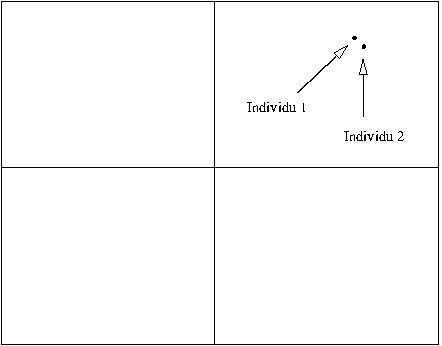
\includegraphics[width = .35\textwidth]{plan_indiv_proche}\\[1ex]
    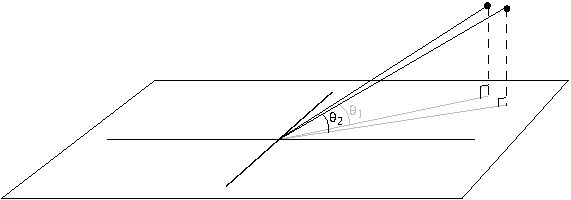
\includegraphics[width = .35\textwidth]{plan_3d_proche}
    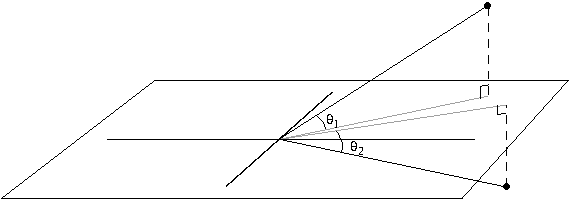
\includegraphics[width = .35\textwidth]{plan_3d_eloigne}
    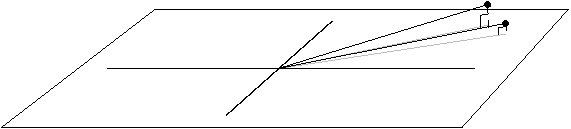
\includegraphics[width = .35\textwidth]{plan_3d_proche2}
    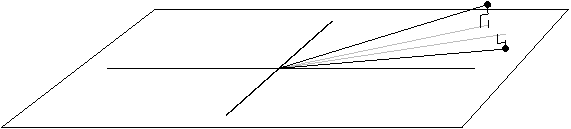
\includegraphics[width = .35\textwidth]{plan_3d_eloigne2}
    \caption{Same projections but different situations {\tiny (source: E. Matzner)}}

  \end{figure}

 $\rightsquigarrow$ Only work when individuals are well represented in the lower space
\end{frame}

\begin{frame}[fragile]
  \frametitle{Individual: quality of the representation}
  
  \begin{block}{Property}
    \begin{itemize}
      \item  An individual $i$ is well represented by $\Delta_k$ if it is close to this axis.
      \item  In other word, vector $\bx_i - \bar{\bx}$ and $\bu_k$ are close to collinear
    \end{itemize}
  \end{block}
 
     We use the cosine of the angle $\theta_{ik}$ between $\bx_i - \bar{\bx}$ and $\bu_k$ to measure the degree of co-linearity:
     \begin{equation*}
       \cos^2(\theta_{ik}) = \frac{\bigg(\bu_k^\top (\bx_i - \bar{\bx})\bigg)^2}{\|\bx_i - \bar{\bx} \|^2 \xout{\|\bu_k \|^2}}
     \end{equation*}

\begin{knitrout}
\definecolor{shadecolor}{rgb}{0.969, 0.969, 0.969}\color{fgcolor}\begin{kframe}
\begin{alltt}
\hlstd{factoextra}\hlopt{::}\hlkwd{get_pca_ind}\hlstd{(crabs_pca)}\hlopt{$}\hlstd{cos2} \hlopt \hlkwd{head}\hlstd{(}\hlnum{3}\hlstd{)} \hlopt \hlkwd{kable}\hlstd{(}\hlstr{"latex"}\hlstd{)}
\end{alltt}


{\ttfamily\noindent\bfseries\color{errorcolor}{\#\# Error in factoextra::get\_pca\_ind(crabs\_pca)\$cos2 \%>\% head(3) \%>\% kable("{}latex"{}): could not find function "{}\%>\%"{}}}\end{kframe}
\end{knitrout}
\end{frame}

\begin{frame}[fragile]
  \frametitle{Individual: contribution to an axis}


  \begin{block}{Property}
    \begin{itemize}
      \item Inertia "explained" by $\Delta_k$ is inertia of $\Delta_k^\bot$
      \item $I_{\Delta_k^\bot} = n^{-1}\sum_{i=1}^n \distance^2(\Delta_k^\bot, \bx_i) $
    \end{itemize}
  \end{block}
 
     Contribution of $\bx_i$ to axis $\Delta_k$ is the proportion of variance/inertia carried by individual $i$:
     \begin{equation*}
       \mathrm{contr} (\bx_i) = \frac{n^{-1}\distance^2(\Delta_k^\bot, \bx_i)}{I_{\Delta_k^\bot}} = \frac{\bigg(\bu_k^\top (\bx_i - \bar{\bx})\bigg)^2}{n\lambda_k} 
     \end{equation*}


\begin{knitrout}
\definecolor{shadecolor}{rgb}{0.969, 0.969, 0.969}\color{fgcolor}\begin{kframe}
\begin{alltt}
\hlstd{factoextra}\hlopt{::}\hlkwd{get_pca_ind}\hlstd{(crabs_pca)}\hlopt{$}\hlstd{contr} \hlopt \hlkwd{head}\hlstd{(}\hlnum{3}\hlstd{)} \hlopt \hlkwd{kable}\hlstd{(}\hlstr{"latex"}\hlstd{)}
\end{alltt}


{\ttfamily\noindent\bfseries\color{errorcolor}{\#\# Error in factoextra::get\_pca\_ind(crabs\_pca)\$contr \%>\% head(3) \%>\% kable("{}latex"{}): could not find function "{}\%>\%"{}}}\end{kframe}
\end{knitrout}
  
\end{frame}

\subsection{Variables point of view}

\begin{frame}
  \frametitle{Cloud of variables in $\Rset^n$}
  
  \begin{center}
    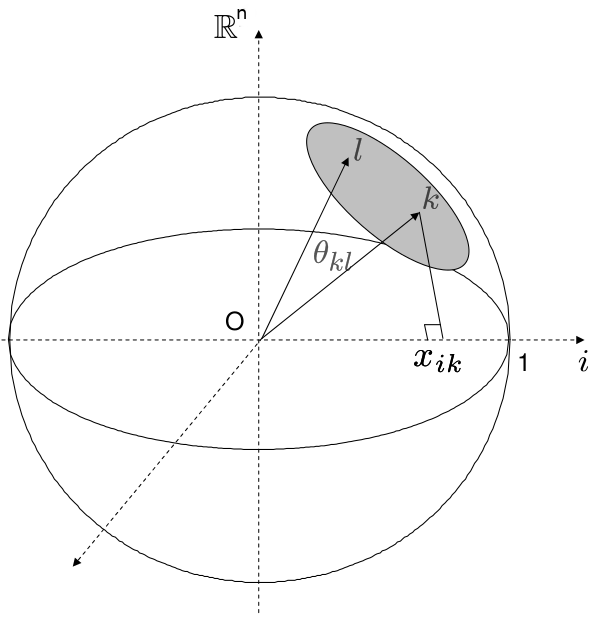
\includegraphics[width=.45\textwidth]{nuage_var}
  \end{center}

  Direct equivalence between geometry and statistics (collinearity $\equiv$ correlation) 
  \begin{equation*}
    \cos(\theta_{kl}) = \frac{\langle \bx^k ,\bx^\ell \rangle}{\|\bx^k\| \|\bx^\ell\|} = \rho(\bx^k,\bx^\ell)
  \end{equation*}

\end{frame}

\begin{frame}
  \frametitle{Principal Components}
  
  \begin{block}{Dual representation}
    A symmetric reasoning can be made in $\Rset^n$ for the variables, like with the individuals in $\Rset^p$.
    
    $\rightsquigarrow$ New axes are linear combinaison of the original variables, which can be seen as \alert{\bf new variables} in the new latent space
  \end{block}

  \begin{block}{Principal component}
    It is the linear combinasion formed by the orginal variables with weights given by the loadings $\bu_k = (u_{k1}, \dots, u_{kj}, \dots, u_{kp})$
    \begin{equation*}
      \mathbf{f}_{k}  = \sum_{j=1}^p u_{kj} (\bx^{j} - \bar{x}_j) = \bX^c \bu_k, \quad \mathbf{f}_k \in \Rset^n
    \end{equation*}
    Sometimes called \alert{"factors"} in  factor analysis, as \alert{latent (hidden) variables}. 
  \end{block}

\end{frame}

\begin{frame}
  \frametitle{Variable representation in the new space}
  
  \begin{block}{Connection with original variables}
    \begin{itemize}
      \item essential for interpretation
      \item answer to the question: how to read the axes of the individual map
      \item use correlation to measure connection to original variable
    \end{itemize}
  \end{block}

  \begin{equation*}
    \var(\mathbf{f}_k) = \frac{1}{n}\var(\bX^c \bu_k) = \bu_k^\top \frac{1}{n}(\bX^c)^\top \bX^c \bu_k =  \bu_k^\top \hat{\bSigma} \bu_k = \lambda_k
  \end{equation*}
  
  \begin{equation*}
    \cov(\mathbf{f}_k, (\bx^j - \bar{x}_j)) = \bu_k \top {\bX^c}^\top \bX^c e_j = \bu_k \lambda_k e_j = \lambda_k \bu_{kj}   
  \end{equation*}

  \begin{equation*}
    \cor(\mathbf{f}_k, (\bx^j - \bar{x}_j)) =  \sqrt{\frac{\lambda_k}{\var(\bx^j)}}\bu_{kj}
  \end{equation*}
  
\end{frame}

\begin{frame}[fragile]
  \frametitle{Variable vizualisation: correlation circle (1)}

\begin{knitrout}
\definecolor{shadecolor}{rgb}{0.969, 0.969, 0.969}\color{fgcolor}\begin{kframe}
\begin{alltt}
\hlkwd{fviz_pca_var}\hlstd{(crabs_pca)}
\end{alltt}


{\ttfamily\noindent\bfseries\color{errorcolor}{\#\# Error in fviz\_pca\_var(crabs\_pca): could not find function "{}fviz\_pca\_var"{}}}\end{kframe}
\end{knitrout}

\end{frame}

\begin{frame}[fragile]
  \frametitle{Variable vizualisation: correlation circle (2)}

\begin{knitrout}
\definecolor{shadecolor}{rgb}{0.969, 0.969, 0.969}\color{fgcolor}\begin{kframe}
\begin{alltt}
\hlkwd{fviz_pca_var}\hlstd{(crabs_pca,} \hlkwc{axes} \hlstd{=} \hlkwd{c}\hlstd{(}\hlnum{2}\hlstd{,}\hlnum{3}\hlstd{))}
\end{alltt}


{\ttfamily\noindent\bfseries\color{errorcolor}{\#\# Error in fviz\_pca\_var(crabs\_pca, axes = c(2, 3)): could not find function "{}fviz\_pca\_var"{}}}\end{kframe}
\end{knitrout}

\end{frame}

\begin{frame}{Warning: about angle after projection}

  \alert{Close projection doesn't mean close variable!}

  \begin{figure}
    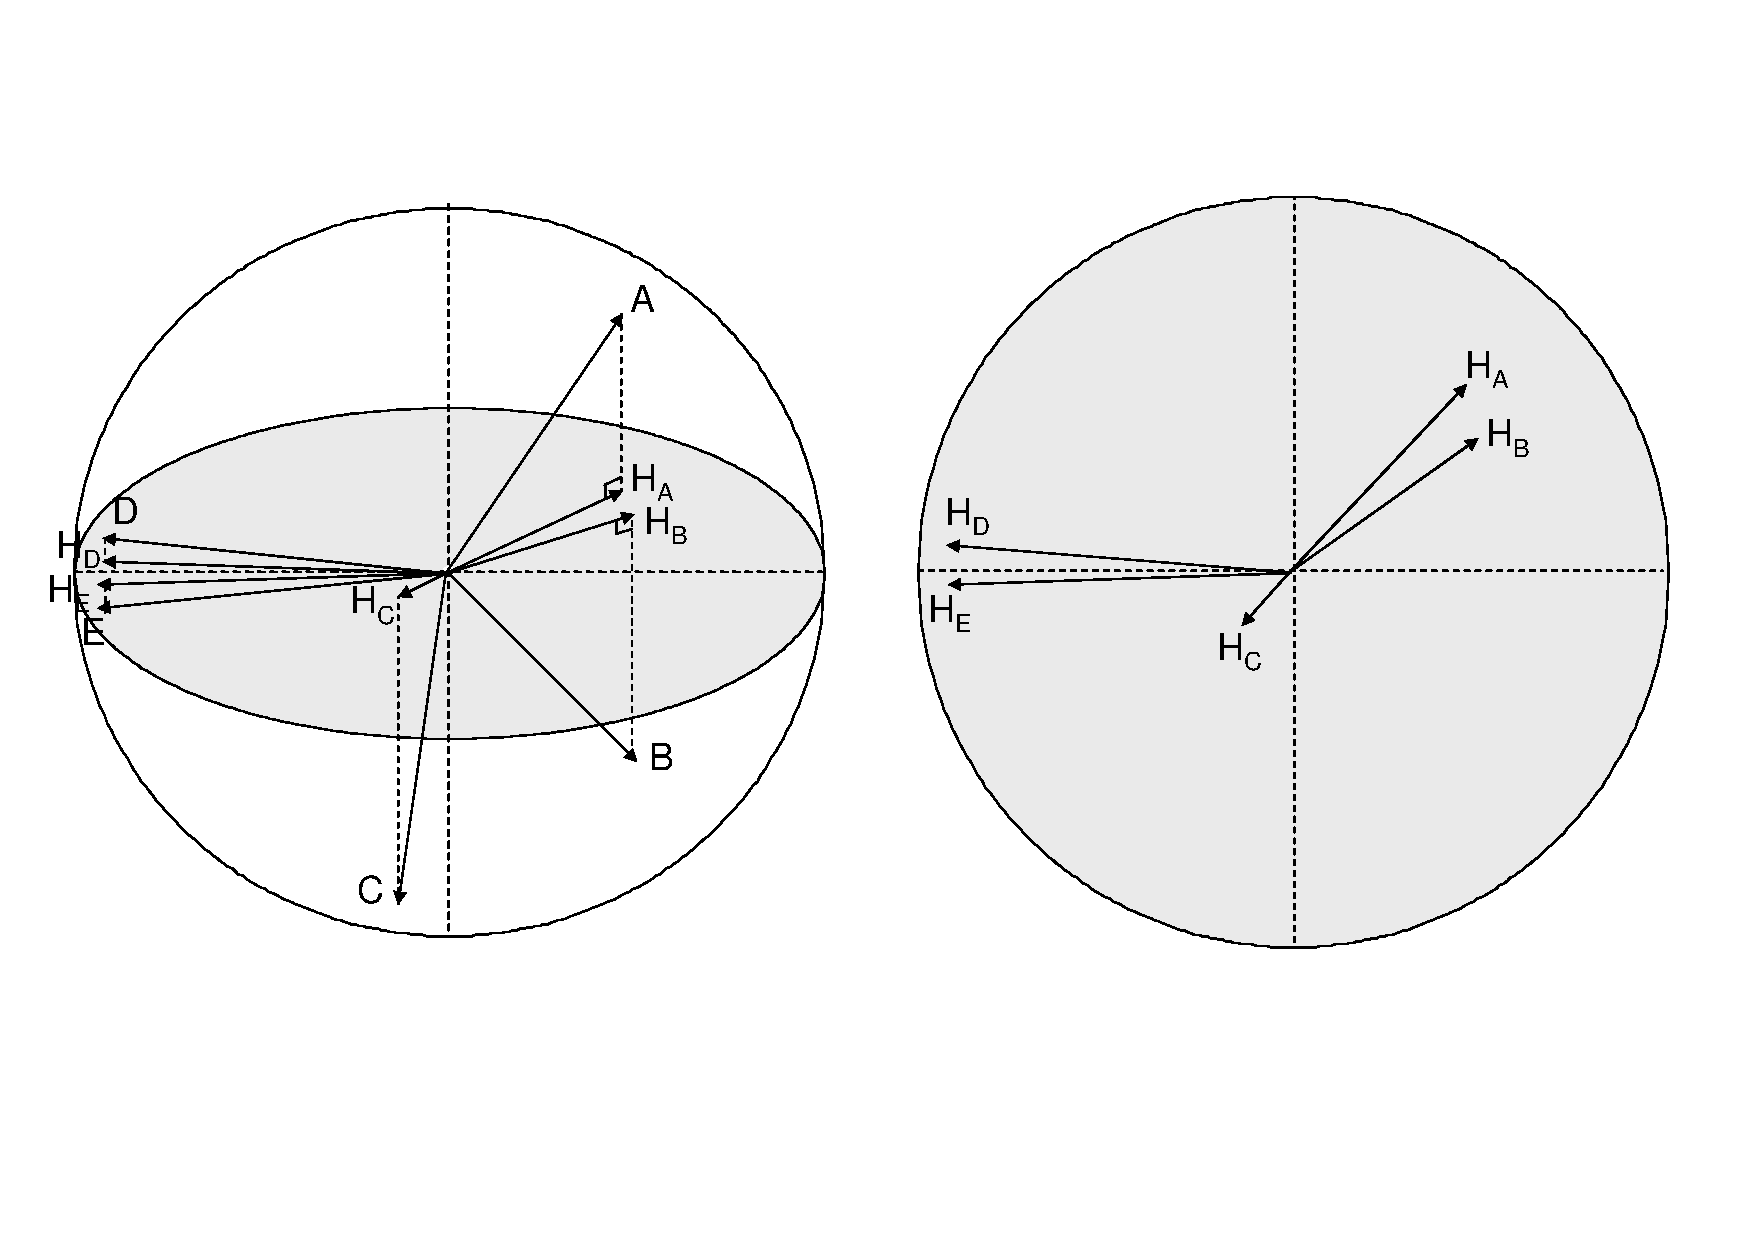
\includegraphics[width = .85\textwidth]{proj_var_acp}
    \caption{Same angle but different situations {\tiny (source: J. Josse)}}

  \end{figure}

 $\rightsquigarrow$ Only work when variables are well represented in the latent space
\end{frame}

\begin{frame}[fragile]
  \frametitle{Variable: quality of the representation}

  Same story as for individuals
  \begin{block}{Property}
    \begin{itemize}
      \item  An variable $j$ is well represented by $\Delta_k$ if its projection is close to $\mathbf{f}_k$.
      \item  High collinearity means high absolute correlation and high cosine.
      \item  use cosine to the square of the angle between the original and new variables.
    \end{itemize}
   $\rightsquigarrow$ The projection of $j$ must be close to the boundardy of the correlation circle
  \end{block}
 
\begin{knitrout}
\definecolor{shadecolor}{rgb}{0.969, 0.969, 0.969}\color{fgcolor}\begin{kframe}
\begin{alltt}
\hlstd{factoextra}\hlopt{::}\hlkwd{get_pca_var}\hlstd{(crabs_pca)}\hlopt{$}\hlstd{cos2} \hlopt \hlkwd{head}\hlstd{(}\hlnum{3}\hlstd{)} \hlopt \hlkwd{kable}\hlstd{(}\hlstr{"latex"}\hlstd{)}
\end{alltt}


{\ttfamily\noindent\bfseries\color{errorcolor}{\#\# Error in factoextra::get\_pca\_var(crabs\_pca)\$cos2 \%>\% head(3) \%>\% kable("{}latex"{}): could not find function "{}\%>\%"{}}}\end{kframe}
\end{knitrout}

\end{frame}

\begin{frame}[fragile]
  \frametitle{Variable: contribution to an axis}
  
  Similarly to individuals, we can measure the contribution of the original variables to the construction of the new ones.
  
\begin{knitrout}
\definecolor{shadecolor}{rgb}{0.969, 0.969, 0.969}\color{fgcolor}\begin{kframe}
\begin{alltt}
\hlstd{factoextra}\hlopt{::}\hlkwd{get_pca_var}\hlstd{(crabs_pca)}\hlopt{$}\hlstd{contr} \hlopt \hlkwd{kable}\hlstd{(}\hlstr{"latex"}\hlstd{)}
\end{alltt}


{\ttfamily\noindent\bfseries\color{errorcolor}{\#\# Error in factoextra::get\_pca\_var(crabs\_pca)\$contr \%>\% kable("{}latex"{}): could not find function "{}\%>\%"{}}}\end{kframe}
\end{knitrout}

\vfill

$\rightsquigarrow$ What do you think of the first axe ?

\end{frame}
